\documentclass[a4paper,utf8]{article}
\pdfoptionpdfminorversion=6
\usepackage{graphicx}
\usepackage[heading,fancyhdr]{ctex}
\usepackage{amsmath,amssymb,geometry,ulem}
\usepackage{array,tabularx,tabulary,mhchem,xspace}
\usepackage{floatrow,subfig,multirow,bigstrut}
\usepackage{siunitx,booktabs,longtable,nameref}
\lineskiplimit=1pt
\lineskip=3pt
\geometry{
    top=25.4mm, 
    left=25mm, 
    right=25mm, 
    bottom=25mm,
    headsep=5.9mm,
}
\ctexset{
    chapter = {
        name = {实验,},
        beforeskip = {-23pt}
    }
}
\newcommand{\fgref}[1]{图~\ref{#1}\xspace}
\newcommand{\seqref}[1]{式~(\ref{#1})}
\newcommand{\expinfo}[6][无]{
    {\zihao{-3}\bfseries\songti
    实验名称:\uline{\hfill\mbox{#2}\hfill} \\[2.9mm]
    学\quad 号:\uline{\makebox[25mm]{#3}}\hfill
    姓\quad 名:\uline{\makebox[25mm]{#4}}\hfill
    班\quad 级:\uline{\makebox[25mm]{#5}} \\[2.9mm]
    合作者:\uline{\makebox[25mm]{#1}} \hfill
    桌\quad 号:\uline{\makebox[25mm]{}}\hfill\makebox[25mm+4em]{}\\[2.9mm]
    指导教师:\uline{\makebox[30mm]{#6}}\hfill\mbox{} \\[2.9mm]
    实验日期:\uline{\makebox[30mm]{}}\hfill\mbox{} \\[58.7mm]
    }
}%\expinfo[合作者]{实验名称}{学号}{姓名}{班级}{指导教师}
\newcommand{\pointingbox}{
    {\zihao{4}\bfseries\songti%
    实验考核\\[3mm]
    \extrarowheight=3mm
    \begin{tabularx}{150mm}{|X|X|X|X|X|}\hline
        \hfil 项目 \hfil  & \hfil 实验预习 \hfil & \hfil 实验过程 \hfil & \hfil 分析与讨论 \hfil & \hfil 总评 \hfil \\[3mm] \hline
        \hfil 评价 \hfil &  &  &  &  \\[3mm] \hline
    \end{tabularx}
    }
}
\newcommand{\derivative}[2]{\frac{\mathrm{d} #1}{\mathrm{d} #2}}
\newcommand{\thinking}[2]{\textbf{#1}\\
答:\begin{minipage}[t]{0.85\textwidth}
    #2
\end{minipage}}

\pagestyle{fancy}
\fancyhf{}
%\fancyhead[C]{材料科学基础实验}
%\fancyfoot[C]{\thepage}
\fancyhead[EC]{\leftmark} \fancyhead[OC]{\rightmark}
\fancyhead[EL,OR]{\thepage}
\fancypagestyle{plain}{\renewcommand{\headrulewidth}{0pt}\fancyhf{}}

\newcounter{Rownumber}
\newcommand*{\Rown}{\stepcounter{Rownumber}\theRownumber}
\newcounter{sample}
\newcommand*{\Sam}{\stepcounter{sample}\thesample}
\newcounter{Fignumber}
\newcommand*{\Fign}{\stepcounter{Fignumber}\theFignumber}

\newcommand*{\resetRown}{\setcounter{Rownumber}{0}}
\newcommand{\qrange}[3]{\qtyrange[range-phrase = \text{$\sim$},range-units =single]{#1}{#2}{#3}}
\floatsetup[table]{capposition=top}
\newcolumntype{C}{>{\hfil}X<{\hfil}}
\renewcommand{\Nameref}[1]{\textbf{\ref{#1}~\nameref{#1}}}
\newcommand{\TTR}[0]{\watt\per\m\per\K} %导入导言
\begin{document}
\begin{center}
    {\mbox{}\\[7em]\zihao{2}\bfseries\songti%
    材料科学基础实验报告}\\[34mm]
    \expinfo{金属材料机械性能测量:拉伸和压缩}{22301077}{张蕴东}{22高分子}{李继玲}
    {\zihao{4}\bfseries\songti
    实验考核\\[3mm]
    \extrarowheight=3mm
    \begin{tabularx}{150mm}{|X|X|X|X|X|}\hline
        \hfil 项目 \hfil  & \hfil 实验预习 \hfil & \hfil 实验过程 \hfil & \hfil 分析与讨论 \hfil & \hfil 总评 \hfil \\[3mm] \hline
        \hfil 评价 \hfil &  &  &  &  \\[3mm] \hline
    \end{tabularx}
    }
\end{center}
\newpage
\part{拉伸实验}
\section{实验目的}
\begin{itemize}
    \item 了解电子万能试验机的基本结构、工作原理及使用方法;
    \item 观察拉伸时所表现的各种现象;
    \item 观察低碳钢和铸铁的断口特征,辨别两种材料的力学特征;
    \item 通过低碳钢和铸铁的应力-应变曲线,评价二者的力学性能,掌握金属材料屈服强度,抗拉强度,断裂伸长率和断面收缩率的测定方法。
\end{itemize}
\section{实验原理}%简单描述,含必要的公式和附图;
\subsection{低碳钢拉伸的应力-应变曲线及特征参数}
\subsubsection{低碳钢拉伸的应力-应变曲线}
低碳钢是塑性材料的典型代表性材料,对于低碳钢试样,在受拉伸过程中,如\fgref{fig:1} 所示应力-应变曲线,可以观察到试样经历四个典型的变形阶段:弹性变形阶段,屈服阶段,均匀塑性变形阶段(强化阶段),局部塑性变形阶段(颈缩阶段),伴随着应力-应变曲线上存在不同的特征点。
\begin{figure}[!ht]
    \begin{floatrow}\centering
        \ffigbox{\caption{低碳钢的拉伸曲线(R-e 曲线)}\label{fig:1}}{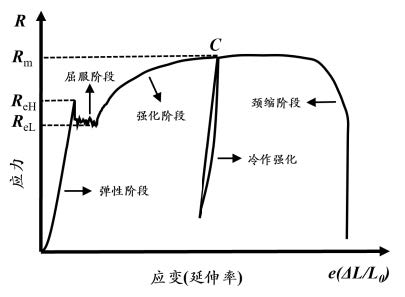
\includegraphics[height=50mm]{1.jpg}}
        \ffigbox{\caption{铸铁的拉伸曲线}\label{fig:2}}{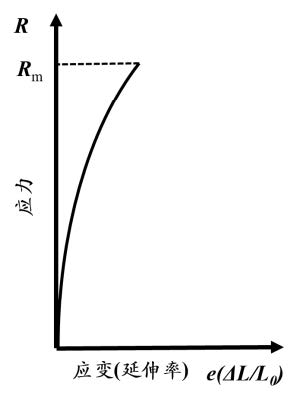
\includegraphics[height=50mm]{2.jpg}}
    \end{floatrow}
\end{figure}
\subsubsection{铸铁的应力-应变曲线}
铸铁是典型的脆性材料,铸铁的拉伸变形无屈服现象和缩颈现象,进行非常小的塑性变形后在较小的应力作用下就可被拉断,且突然断裂。拉断后铸铁的延伸率通常很小,约为 0.5\%。\fgref{fig:2} 为铸铁典型的应力-应变曲线,由图可见,铸铁的应力-应变曲线没有明显的直线部分。铸铁拉断前承受的最大应力值为其被拉伸的强度极限,定义为铸铁的抗拉强度。
\subsection{相关概念基本定义及计算公式}
\noindent 弹性模量:在应力-应变曲线上,应力低于弹性极限的范围内,应力与应变的比值,表达式为:\linebreak $E =\displaystyle \frac{\sigma}{\varepsilon}$ ,$\sigma$ 为应力,$\varepsilon$ 为应变。\\
上屈服强度 $R_{eH}$:试样发生屈服时应力下降时达到的最大值。\\
下屈服强度 $R_{eL}$:试样屈服期间屈服平台上不计初始屈服瞬时效应的最低应力点。\\
抗拉强度 $R_m$:试样缩颈前所达到的最大应力值。\\
原始标距 $L_0$:试样初始状态,夹头内用于测试的等截面积的试样部分的长度。\\
断后标距 $L_u$:实验被拉断后,将试样断口处紧密对接,初始标线内的总长度。\\
断后延伸率 $\delta$:试样拉断后,试样原始标线之间的伸长量和原始标距之比,$\delta = \displaystyle\frac{L_u-L_0}{L_0}\times 100\%$。\\
断面收缩率 $\psi$:试样拉断后,断口处横截面积的最大缩小量与原始标距内截面积之比,\linebreak $\psi = \displaystyle\frac{L_0-L_u}{L_0}\times 100\%$。
\section{实验仪器}%规格及参数
电子万能试验机,控制微机,游标卡尺,YYU-25/50 电子引伸计,低碳钢标准试样,铸铁标准试样。
\section{实验过程}%简述主要过程和实验内容
\begin{enumerate}
    \item 首先,在装夹试样前,标记待测试样的原始标距 $L_0$。选取待测试样夹头内部变形部分偏中间位置,在此处不同位置处选择3~5个截面,用游标卡尺在每个截面相互垂直的两个方向上分别测量一次该截面的直径,对所测量的所有截面直径求平均值即可视为待测试样拉伸之前的直径,记为 $d_0$,之后在待测试样夹头中间变形部分,以其变形部分的中点为中心,左右各选取 $5d_0$ 共 $10d_0$ 的长度,在端点处做标记,标记内即为待测试样的原始标距 $L_0$。
    \item 检查并确认电子万能试验机和计算机已连接。之后打开万能电子试验机,旋转红色急停旋钮使其弹起。
    \item 安装拉伸模具。
    \item 装夹试样。
    \item 装夹引伸计(低碳钢拉伸)。
    \item 编辑实验方案进行并进行测量。
    \item 进行测试
    \item 测量断后试样尺寸
    \item 保存数据,作图并分析待测试样各力学性能参数指标。
    \item 测量铸铁的拉伸曲线。
    \item 根据测量的低碳钢和铸铁的拉伸曲线,分析和判断两类金属材料的力学性能和各性能指标参数。
\end{enumerate}

\newpage
\part{压缩实验}
\setcounter{section}{0}
\section{实验目的}
    \begin{itemize}
        \item 测定低碳钢在压缩时的名义屈服强度 $R_\text{pc0.2}$;
        \item 测定铸铁在压缩时的强度极限 $R_m$;
        \item 观察上述材料在压缩时的变形及破坏形式,并分析其破坏原因;
        \item 比较塑性材料与脆性材料的力学性能及特点。
    \end{itemize}
\section{实验原理}%简单描述,含必要的公式和附图;
    \subsection{低碳钢}
        低碳钢为塑性材料,其压缩曲线($F$-$\Delta L$ 曲线)如\fgref{fig:4} 所示,开始加载时,力-变形曲线呈直线上升,此时材料服从胡克定律。当载荷达到一定值以后,随载荷增加变形加快,不再为线性关系,但试样无明显屈服现象。随载荷进一步增大,曲线逐渐向上弯曲。这是因为随着塑性变形的迅速增长,试样横截面积逐渐增大,增加了承载能力,同时纵向变形速度下降,从而导致力-变形关系曲线上翘。
        \begin{figure}[!ht]
            \subfloat[\mbox{}]{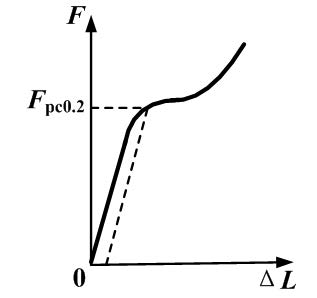
\includegraphics[height=35mm]{4.jpg}\label{fig:4}}\hspace{10mm}
            \subfloat[\mbox{}]{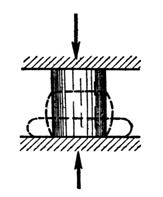
\includegraphics[height=35mm]{5.jpg}}
            \caption{低碳钢压缩图}
        \end{figure}
        \subsection{铸铁}
            铸铁为脆性材料,其压缩曲线在开始时接近直线。随载荷增加曲率逐渐增大,最后至破坏,破坏后试件的断面法线方向与轴线夹角 $\alpha$ 大约为 $45^\circ$-$55^\circ$。\par
            如\fgref{fig:5a} 所示,铸铁没有屈服极限,只有在最大载荷 $F_m$ 下测出的强度极限 $R_m$。铸铁的抗压强度极限比它的抗拉强度极限高 $3\sim4$ 倍。其它脆性材料,如混凝土、石料等的抗压强度也远高于相应材料的抗拉强度。
            \begin{figure}[!ht]
                \subfloat{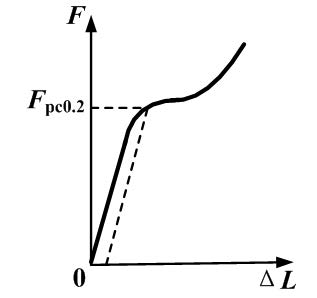
\includegraphics[height=35mm]{4.jpg}}\hspace{10mm}
                \subfloat{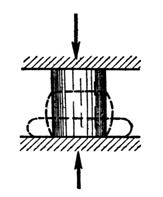
\includegraphics[height=35mm]{5.jpg}}
                \caption{铸铁压缩图}\label{fig:5a}
            \end{figure}
\section{实验仪器}%规格及参数
    \begin{enumerate}
        \item 实验所采用的设备及工具与拉伸实验相同。
        \item 压缩模具。
        \begin{figure}[!ht]
            \caption{压缩模具}
            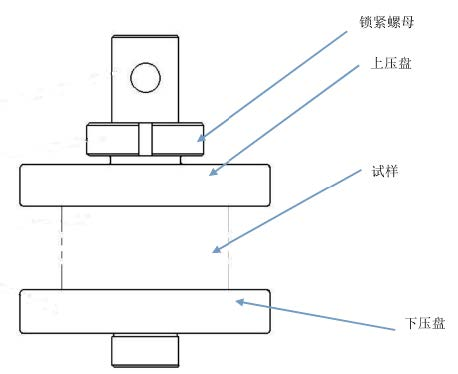
\includegraphics[height=40mm]{3.jpg}
        \end{figure}
    \end{enumerate}
\section{实验过程}%简述主要过程和实验内容
    \begin{enumerate}
        \item 用游标卡尺在互相垂直方向,两次测量金属材料试件的直径,取其平均值为 $d_0$(用于计算试件原始截面面积 $S_0$),同时测量试件高度 $h$(测一次即可)。
        \item 打开设备
        \item 设置试验方案
        \item 装夹试样
        \item 开始测试
        \item 实验结束,将横梁上升,取出被测试样;点击“预览”生成测试结果报告并保存;
    \end{enumerate}
\section{实验结果}
    \subsection{低碳钢}
        根据设备采集到的数据,绘制以下曲线:\newpage
        \begin{figure}[!ht]
            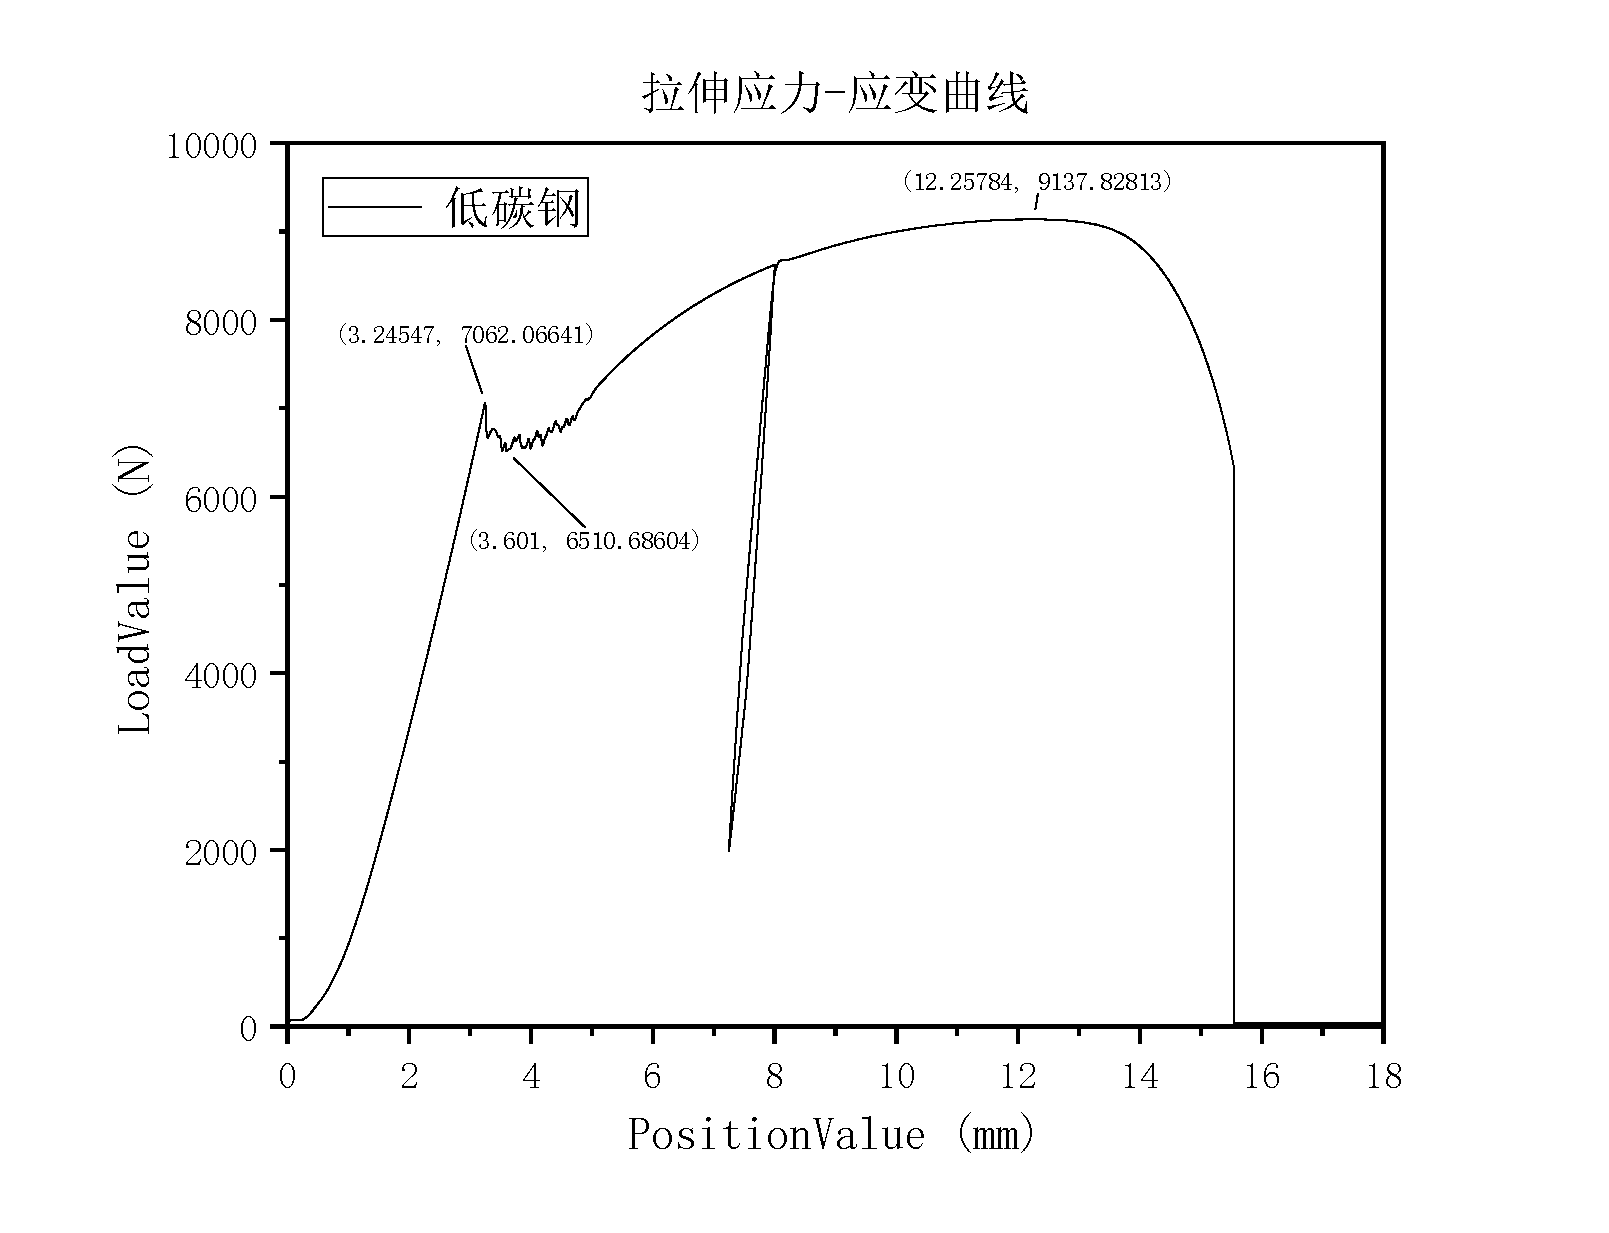
\includegraphics[width=0.8\textwidth]{result/fig1a.pdf}
            \caption{低碳钢拉伸图}
        \end{figure}
        \par
        \begin{figure}[!ht]
            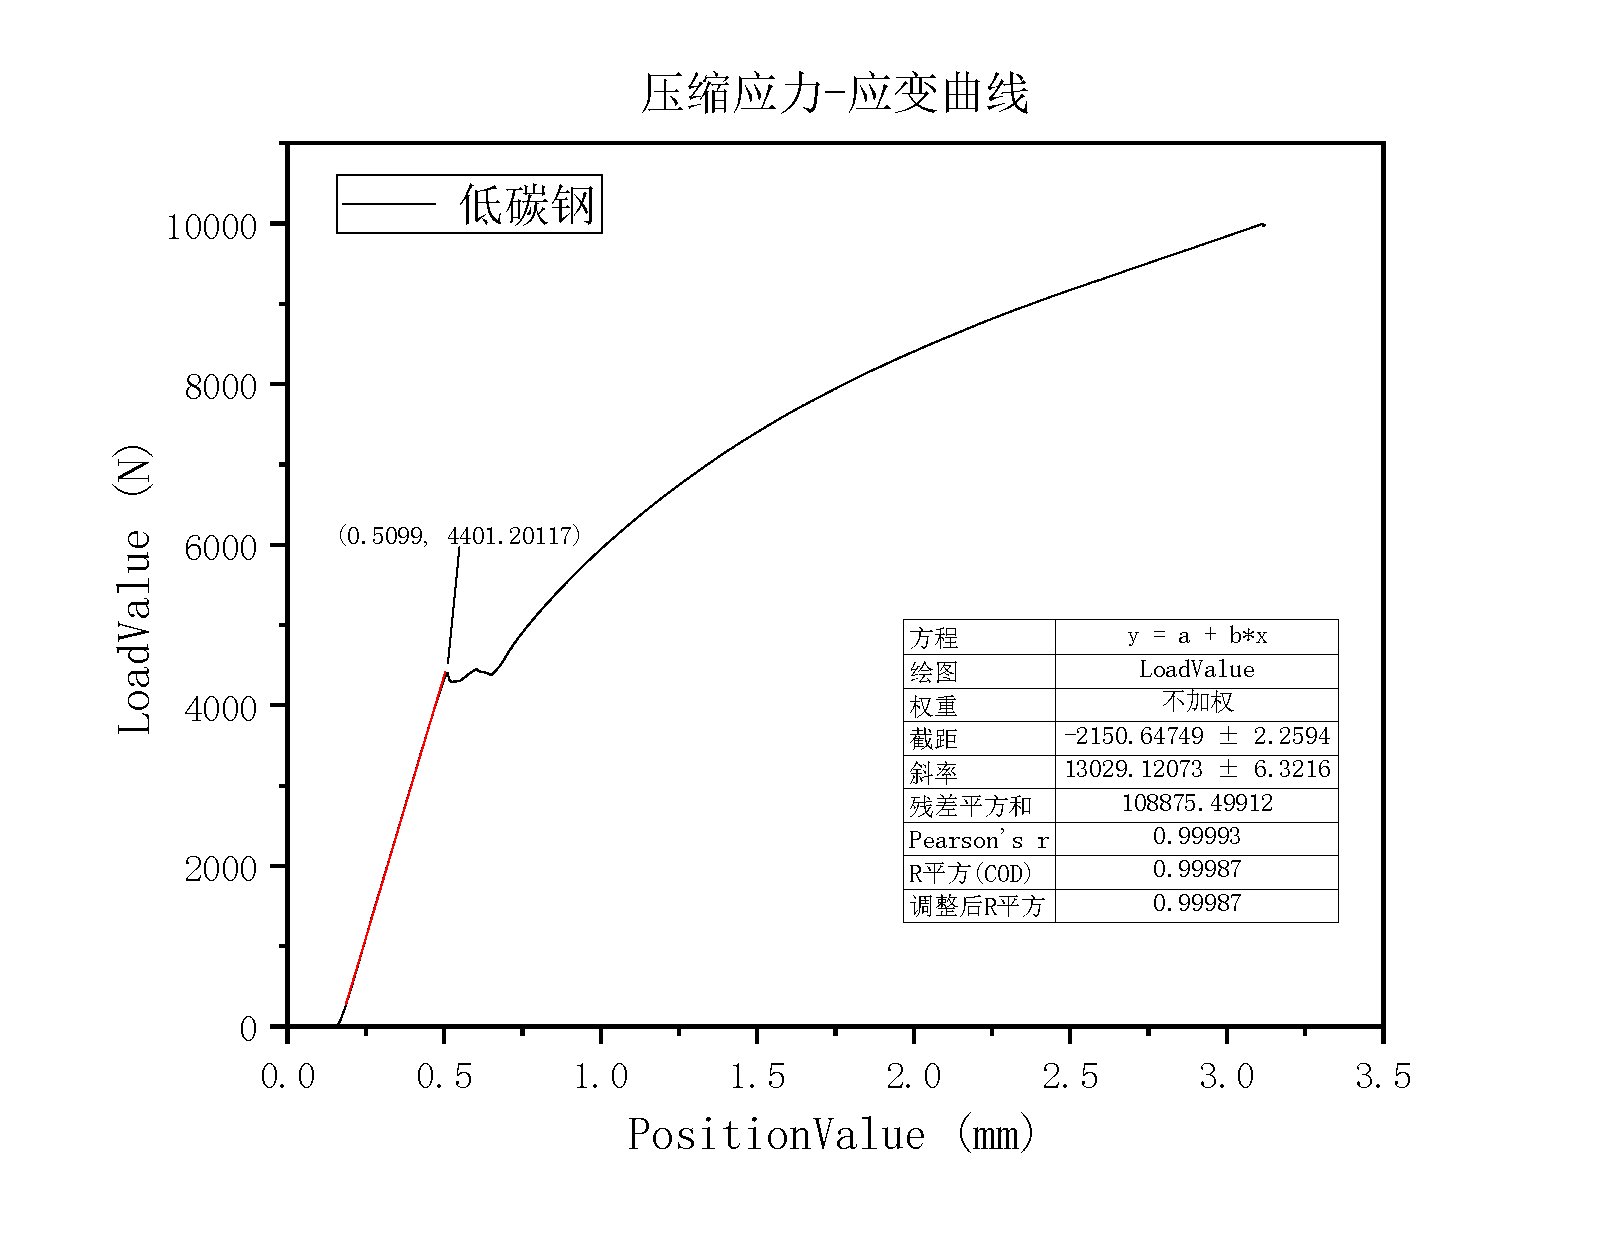
\includegraphics[width=0.8\textwidth]{result/fig1b.pdf}
            \caption{低碳钢压缩图}
        \end{figure}
        实验前后低碳钢的参数变化如下表:\newpage
        \begin{table}[!ht]
            \centering\begin{tabular}{c c c}\hline
                 \ & 直径 $\bar{d}$ & 标距 $\bar{L}$ \\ \hline
                拉伸前 & \SI{4.98}{\mm} & \SI{50.00}{\mm} \\ 
                拉伸后 & \SI{2.83}{\mm} & \SI{61.10}{\mm} \\ \hline
                \ & 直径 $\bar{d}$ & 高度 $\bar{h}$ \\ \hline
                压缩前 & \SI{4.00}{\mm} & \SI{8.00}{\mm} \\ 
                压缩后 & \SI{4.66}{\mm} & \SI{5.68}{\mm} \\ \hline
                拟合直线方程 & $y=13029.12 x - 2150.65$ & $R^2=0.99987$ \\
            \end{tabular}
        \end{table}\par
        由此可以计算出低碳钢的一些力学参数:
        \begin{align*}
            \text{断后延伸率:} A_1 & = \frac{L_1-L_0}{L_0} (\%) = 22.20 \% \\
            \text{断后收缩率:} Z_1 & = \frac{\Delta d^2}{{d_0}^2} (\%) = 67.71 \% \\
            \text{上屈服强度:} R_{eH1} & = \frac{F_{eH1}}{S_0} = \SI{359.668}{\MPa}\\
            \text{下屈服强度:} R_{eL1} & = \frac{F_{eL1}}{S_0} = \SI{331.587}{\MPa}\\
            \text{抗拉强度:} \sigma_1 & = \frac{F_1}{S_0} = \SI{465.385}{\MPa} \\
            \text{抗压强度:} {\sigma^{'}}_1 & = \frac{F_1}{S_0} = \SI{224.151}{\MPa}\\
        \end{align*}

    \subsection{铸铁}
    实验前后铸铁的参数变化如下表:\par
        \begin{table}[!ht]
            \centering\begin{tabular}{c c c}\hline
                \ & 直径 $\bar{d}$ & 标距 $\bar{L}$ \\ \hline
                拉伸前 & \SI{4.91}{\mm} & \SI{49.30}{\mm} \\ 
                拉伸后 & \SI{4.81}{\mm} & \SI{49.40}{\mm} \\ \hline
                \ & 直径 $\bar{d}$ & 高度 $\bar{h}$ \\ \hline
                压缩前 & \SI{3.75}{\mm} & \SI{7.86}{\mm} \\ 
                压缩后 & \SI{4.10}{\mm} & \SI{6.78}{\mm} \\ \hline
            \end{tabular}
        \end{table}\par
        根据设备采集到的数据,绘制以下曲线:\newpage
        \begin{figure}[!ht]
            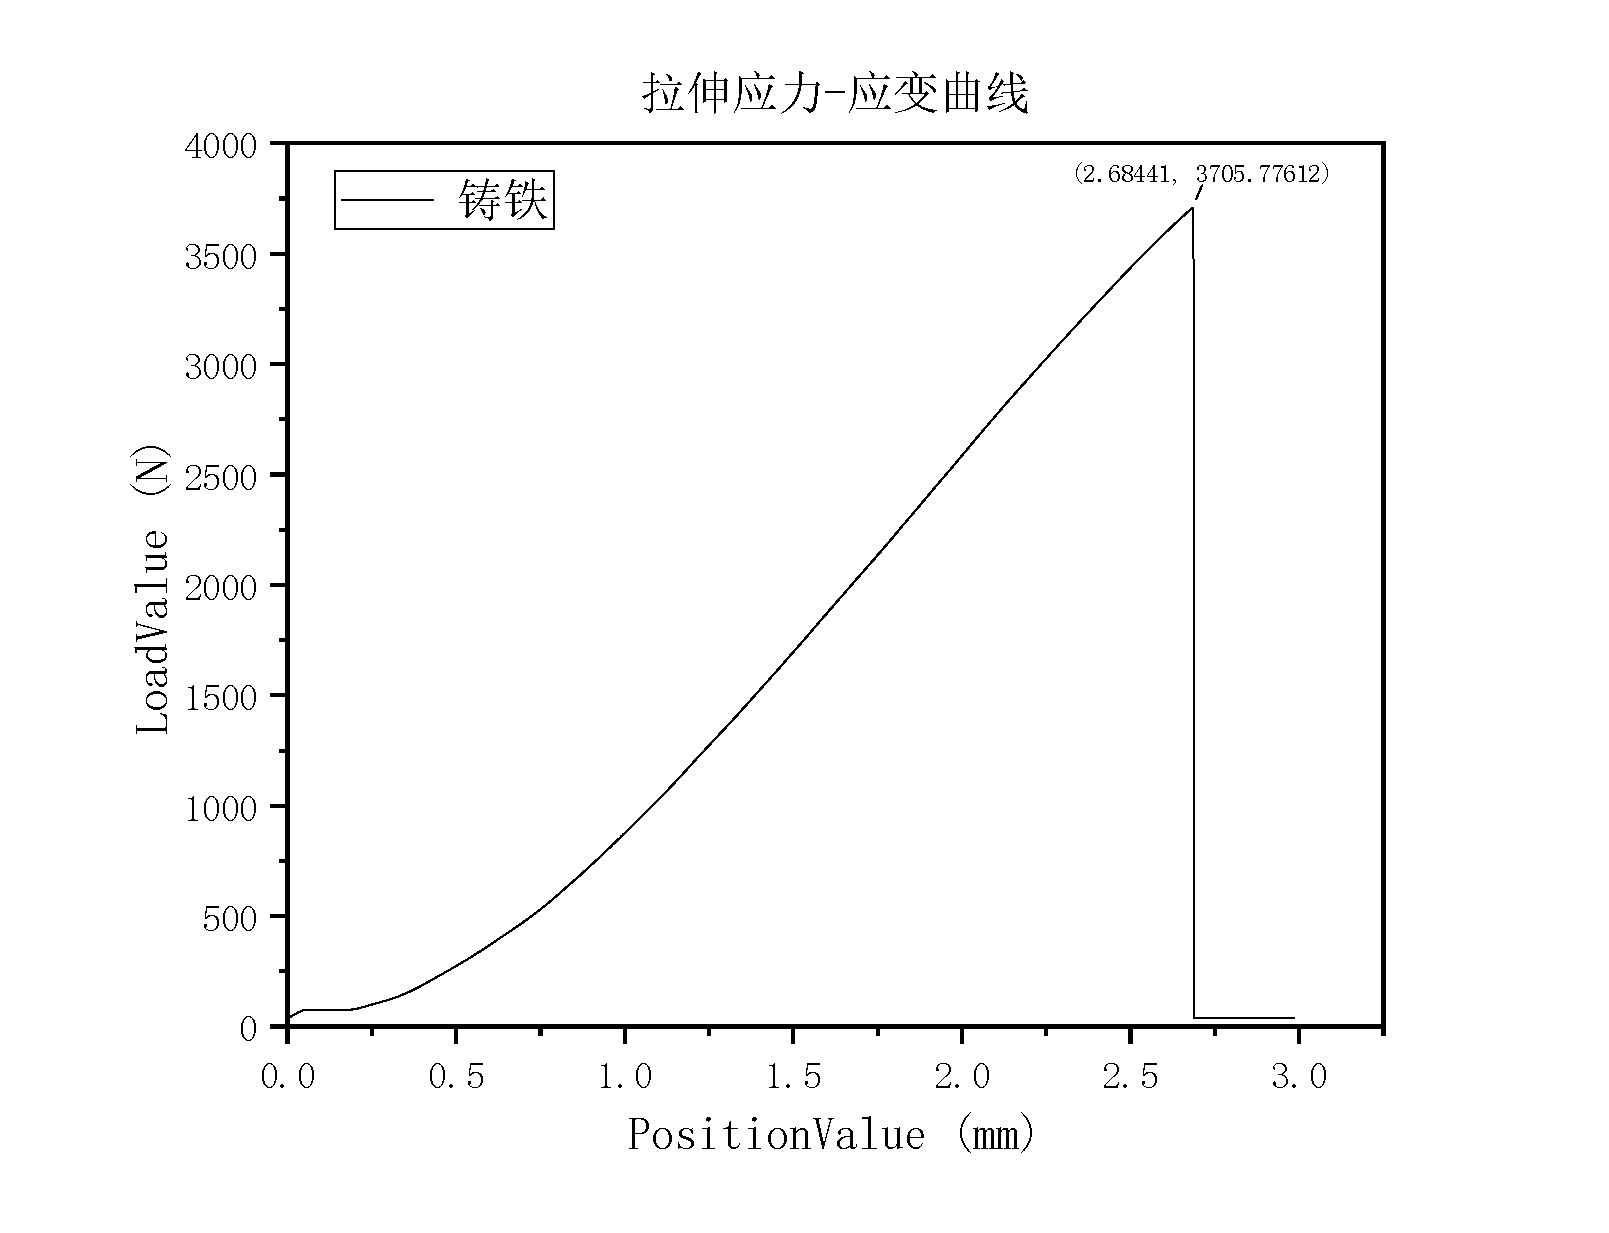
\includegraphics[width=0.8\textwidth]{result/fig2a.pdf}
            \caption{铸铁拉伸图}
        \end{figure}
        \begin{figure}[!ht]
            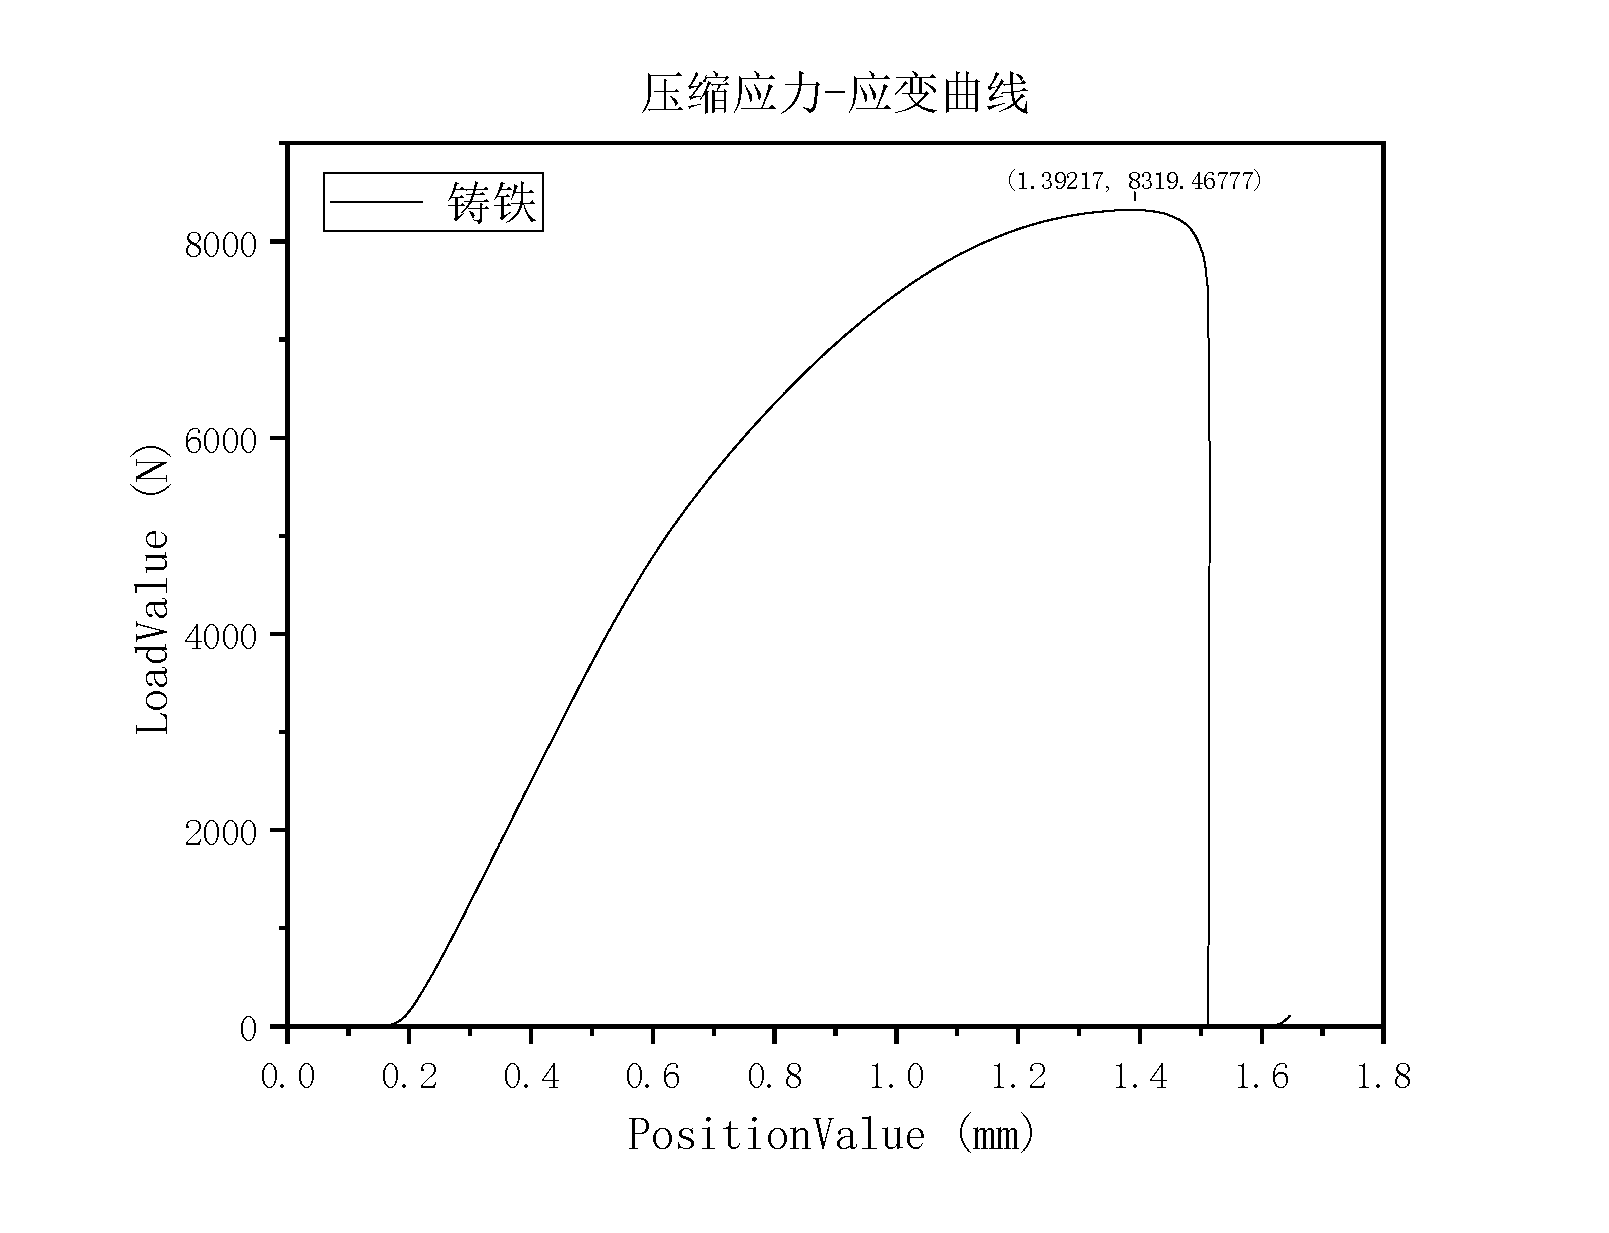
\includegraphics[width=0.8\textwidth]{result/fig2b.pdf}
            \caption{铸铁压缩图}
        \end{figure}
        
        由此可以计算出铸铁的一些力学参数:
        \newpage
        \begin{align*}
            \text{断后延伸率:} A_2 & = \frac{L_1-L_0}{L_0} (\%) = 0.20 \% \\
            \text{断后收缩率:} Z_2 & = \frac{\Delta d^2}{{d_0}^2} (\%) = 4.03 \% \\
            \text{抗拉强度:} \sigma_2 & = \frac{F_2}{S_0} = \SI{188.734}{\MPa} \\
            \text{抗压强度:} {\sigma^{'}}_2 & = \frac{F_2}{S_0} = \SI{689.340}{\MPa}\\
        \end{align*}
\subsection{不确定度分析}
    \subsubsection{A 类不确定度分量的评估}
    对一个随机变量 $x$ 进行了 $n$ 次重复测量,其算术平均值 $\bar{x}$ 作为对被测量 $x$ 的最佳统计评估值,平均值的标准偏差 $s(\bar{x})$ 作为实验结果的标准不确定度,自由度 $\nu=n-1$。计算公式为\\
    \begin{align}
        \bar{x}&=\frac{1}{n}\sum_{i=1}^{n}x_i \label{exp:amean} \\
        s(\bar{x})&=\sqrt{\frac{1}{n(n-1)}\sum_{i=1}^{n}(x_i-\bar{x})^2} \label{exp:astd}
    \end{align}

    \subsubsection{B 类不确定度分量的评估}
    对一个非重复测量得到的量 x 进行不确定度分析时,评估者需根据已获得的信息人为假定其服从某种概率分布来评估其方差 $u^2(x)$ 或标准不确定度 $u(x)$。具体步骤是,首先根据量 $x$ 的变化范围确定其半宽度 $a$,然后根据假定的概率分布计算标准不确定度。\\
    \begin{equation}
        u(x) = \frac a k \label{exp:uncertaintyB}
    \end{equation}
    在 100\% 和 95\% 置信概率下,矩形分布时的包含因子 $k$ 值分别为 $\sqrt{3}$ 和 $1.65$,三角形分布时的包含因子 $k$ 值分别为 $\sqrt{6}$ 和 $1.90$,正态分布时的包含因子 $k$ 值分别为 $3$ 和 $1.96$。

    \subsubsection{直接测量量的合成标准不确定度}
    直接测量量的合成标准不确定度 $u_c(x)$ 由其 A 类标准不确定度分量 $s(\bar{x})$ 与其 B 类标准不确定度分量 $u(x)$ 采用方和根法合成,即\\
    \begin{equation}
        u_c(x) = \sqrt{s^2(\bar{x})+u^2(x)} \label{exp:uncertaintyCombine}
    \end{equation}
    合成标准不确定度 $u_c$ 的自由度称为有效自由度,用 $\nu_\text{eff}$ 表示。当各分量间相互独立且合成量接近正态分布或 t 分布时,有效自由度 $\nu_\text{eff}$ 可以由下面的韦尔奇-萨特韦特(Welch-Satterthwaite)公式计算\\
    \begin{equation}
        \nu_\text{eff}=\frac{u_c^4(x)}{\displaystyle\frac{s^4(x)}{\nu_\text{A}}+\frac{u^4(x)}{\nu_\text{B}}} \label{exp:validFreedom}
    \end{equation}
    式中 $\nu_\text{A}$ 和 $\nu_\text{B}$ 分别是 A 类和 B 类标准不确定度分量对应的自由度数。如果 $\nu_\text{eff}$ 不是整数,则去掉小数部分取整,即将 $\nu_\text{eff}$ 取为一个不大于 $\nu_\text{eff}$ 本身的整数。

    \subsubsection{标准不确定度的传播规律}
    标准不确定度传播规律的数学基础是全微分。假设间接测量量 $y$ 与直接测量量 $x_1$, $x_2$, $x_3$, $\cdots$, $x_n$ 满足函数关系 $y = f(x_1,x_2,x_3,\cdots,x_n)$,且各个直接测量量 $x_1$, $x_2$, $x_3$, $\cdots$, $x_n$ 是相互独立的。对于以标准偏差表示的标准不确定度,需以方和根的形式求和,因此,当各个直接测量量依次有 $u(x_1)$, $u(x_2)$, $u(x_3)$, $\cdots$, $x_n$ 的标准不确定度时,间接测量量 $y$ 的标准不确定度 $u_c(y)$ 可以表示为\\
    \begin{equation}
        u_c^2(y)=\sum_{i=1}^{n}\left[\frac{\partial f}{\partial x_i}\right]^{2}u^2\left(x_{i}\right)=\sum_{i=1}^{n}c_i^2 u^2\left(x_{i}\right) \label{exp:uncertaintyPropagation}
    \end{equation}
    间接测量量 $y$ 的有效自由度由下式计算\\
    \begin{equation}
        \nu_\text{eff}=\frac{u_c^4(y)}{\displaystyle\sum_{i=1}^{n}\frac{c_i u^4(x_i)}{\nu_i}} \label{exp:validFreedom2}
    \end{equation}

    当需要评定扩展不确定度 $U$ 时,可根据合成标准不确定度的有效自由度 $\nu_\text{eff}$ 和给定的置信概率(譬如 95\%),通过查 t 分布表得出包含因子 $k$,进而给出扩展不确定度 $U = k u_c$。

    \subsection{不确定度计算结果}
    低碳钢:\par
    \begin{align*}
        \text{断后延伸率:} A_1 & = (22.20 \pm 0.56) \% \\
        \text{断后收缩率:} Z_1 & = (67.71 \pm 0.47) \% \\
    \end{align*}\par
    低碳钢:\par
    \begin{align*}
        \text{断后延伸率:} A_2 & = (0.20 \pm 0.11) \% \\
        \text{断后收缩率:} Z_2 & = (4.03 \pm 0.15) \% \\
    \end{align*}\par
    其余量因为不能确定仪器的不确定度分布而难以计算。
    \subsection{结果分析}
    本次实验得到的数据均与理论值吻合较好、但在直径测量上由于颈缩和试样本身不均、导致不确定度较大。当然,其它因素也会影响到结果的准确性,诸如测量数据时的精度,加载应力时的均匀程度之类仪器本身的误差,以及用游标卡尺测量直径和长度时精度带来的误差。
\section{思考题}
\begin{enumerate}
    \item 比较低碳钢和铸铁的拉伸曲线,讨论其差异。
        \begin{enumerate}
            \item 比较本实验低碳钢和铸铁的拉伸曲线可知:低碳钢通常比铸铁具有更
            高的拉伸强度。这是因为低碳钢具有更均匀的结晶结构和较少的缺陷,使其具有
            更高的抗拉性能。
            \item 根据曲线可以看出,低碳钢的图像出现了一段水平锯齿状的曲线,此时低碳钢发生塑性形变而不会立即断裂。相比之下,铸铁则没有这个阶段,更容易发生脆性断裂。
            \item 变形硬化阶段:在继续施加应力时,材料会变得越来越难以变形,这是由于材料内部结构的变化导致的。在这个阶段,应变速率减小,但应变仍在增加,最终导致断裂。
        \end{enumerate}
    \item 低碳钢在拉伸过中可分为几个阶段,各阶段有何特征?\par
        \begin{enumerate}
            \item 弹性阶段:在这个阶段,应力和应变成正比,符合胡克定律。当拉伸力作用停止后,试样能够完全恢复原状,不会留下任何形变。这个阶段的特征是应变与应力成正比,材料在受力时表现为弹性变形,应变能全部恢复。
            \item 屈服阶段:当应力继续增大时,材料会达到一定的应力值,称为屈服点。在屈服点之前,应力与应变成正比,但在屈服点后,应变开始增加但应力不增加,材料发生塑性变形。在这个阶段,试样会发生永久性变形,即使停止受力也不会完全恢复原状。
            \item 屈服后硬化阶段:在超过屈服点后,材料会经历硬化阶段。尽管材料仍然发生塑性变形,但其抗拉强度继续增加,这是由于在变形过程中形成了更多的位错,导致材料内部更加强化。
            \item 变形断裂阶段:在继续施加应力时,材料开始在局部区域发生颈缩,这是由于材料内部结构的变化集中在这些区域。在这个阶段,应变速率减小,但应变仍在增加,最终导致断裂。
        \end{enumerate}
    \item 何谓“冷作硬化”现象?此现象在工程中如何运用?\par
    "冷作硬化"是指在常温下对金属材料进行塑性变形(例如拉伸、压缩、弯曲等),导致其硬度、强度和抗拉弯性能提高的现象。这种硬化是由于金属晶粒在变形过程中发生滑移和再结晶等微观结构变化所致。\par
    在工程中,冷作硬化现象可以用于改善材料的机械性能,例如增加金属的强度、硬度和抗拉弯性能。这种方法可以用于生产高强度、高硬度的零件或制品,如汽车零件、建筑结构、航空航天部件等。冷作硬化还可以用于调节金属材料的弹性模量和导电性能等特性,使其更适用于特定的工程应用。但过度的冷作硬化可能会导致材料变脆,降低其韧性和抗冲击性能,因此在工程设计中需要权衡利弊。

    \item 试分析低碳钢和铸铁试件在压缩过程中及破坏后有哪些区别。\par
    低碳钢和铸铁在压缩过程中及破坏后有许多区别,主要包括以下几个方面:
    \begin{enumerate}
        \item 形变行为:在压缩加载下,低碳钢通常会表现出更多的塑性变形能力,可以发生较大的塑性变形,而铸铁的塑性较差,容易出现脆性断裂。
    
        \item 破坏形态:低碳钢在受到压缩力作用时,通常会发生均匀的塑性变形,最终可能会出现局部的颈缩现象,但整体上会保持一定的连续性;而铸铁在受到压缩力作用时,由于其较差的塑性,容易在应力集中的区域发生裂纹扩展,最终可能呈现出明显的断裂表面。
    
        \item 应力应变曲线:低碳钢在压缩加载下的应力应变曲线通常会比较平缓,在达到极限强度前会有明显的应变硬化阶段;而铸铁的应力应变曲线往往会比较陡峭,在达到极限强度前可能会表现出较少的应变硬化。
    
        \item 能量吸收能力:由于低碳钢具有较好的塑性,因此在压缩过程中能够吸收较多的变形能量,而铸铁的能量吸收能力较低。
    
        \item 微观结构变化:低碳钢在压缩加载过程中,晶粒可能会发生滑移和再结晶等变化,而铸铁中的石墨颗粒会对应力分布产生影响,导致其微观结构的变化。
    \end{enumerate}
    综上所述,低碳钢和铸铁在压缩过程中及破坏后的表现有很大的区别,主要表现在塑性、破坏形态、应力应变曲线、能量吸收能力和微观结构变化等方面。
    \item 与拉伸实验相比较,分析低碳钢和铸铁在压缩时的破坏原因。\par
    低碳钢在压缩过程中,低碳钢通常会表现出更多的塑性变形能力。当受到压缩力时,钢材会发生塑性变形,晶粒会发生滑移和再结晶,使得材料可以更充分地吸收能量。低碳钢在压缩时的破坏通常是由于材料内部的局部应力集中导致的,可能会出现塑性变形过大、局部失稳等情况,最终导致材料的断裂。相比之下,铸铁在压缩时通常会表现出更脆的特性。铸铁的微观结构中含有大量的石墨片或球状石墨,这些石墨会成为应力集中的点,导致材料容易发生裂纹。因此,铸铁在受到压缩力作用时,容易出现裂纹扩展和断裂,而不像低碳钢那样具有较强的塑性变形能力。
    \item 为什么低碳钢压缩时测不出强度极限?\par
    低碳钢在压缩时测不出强度极限的主要原因是由于其在压缩加载下的变形行为与拉伸加载下有所不同。
    \begin{enumerate}
        \item 形变模式不同:在拉伸加载下,材料会逐渐拉长,最终导致断裂。而在压缩加载下,材料的形变模式更加复杂,可能包括挤压、弯曲、局部压扁等形变。这些复杂的形变模式使得难以精确测定强度极限。
        \item 局部应力集中:在压缩加载下,材料内部可能会出现局部应力集中的现象,特别是在材料表面或缺陷处。这会导致在局部区域出现较高的应力,从而导致材料的局部变形和破坏,而不是整体性的断裂,使得测定强度极限变得困难。
        \item 样品几何影响:在拉伸试验中,样品的几何形状相对简单,可以较容易地测定强度极限。而在压缩试验中,样品的几何形状可能更加复杂,如柱形、板材等,这会对应力和应变的分布产生影响,增加了测定强度极限的难度。
    \end{enumerate}
    综上所述,低碳钢在压缩加载下由于其复杂的形变模式、局部应力集中以及样品几何等因素的影响,导致难以准确测定其强度极限。
    \item 简述低碳钢和铸铁的力学性能的主要区别。\par
    低碳钢和铸铁在力学性能上有许多区别,主要包括以下几个方面:
    \begin{enumerate}
        \item 强度和硬度:一般情况下,低碳钢的强度和硬度要高于铸铁。这是因为钢是由铁和一定量的碳组成,碳的添加可以提高钢的硬度和强度,而铸铁中的碳含量较高,但是大部分以石墨的形式存在,对硬度和强度的提升作用有限。
        \item 塑性:低碳钢通常具有较好的塑性,可以在受力时发生较大的塑性变形,而铸铁的塑性较差,容易发生断裂。
        \item 韧性:低碳钢的韧性一般也会比铸铁好,韧性可以指材料在受冲击或振动等作用下不易断裂的性质。
        \item 热处理性能:由于铸铁中含有较高的碳和其他合金元素,使得铸铁的热处理性能较差,一般不能像钢那样进行淬火等热处理,而低碳钢则可以通过热处理来改善其性能。
        \item 耐磨性:由于铸铁中的石墨颗粒可以起到润滑作用,使其具有较好的耐磨性,而低碳钢的耐磨性一般较差。
    \end{enumerate}
    总的来说,低碳钢具有较高的强度、硬度和塑性,适用于要求较高强度和较好塑性的场合;而铸铁具有较好的耐磨性和润滑性,适用于要求耐磨性和润滑性的场合。
\end{enumerate}
\end{document}
